\chapter{Related Work}
\label{cha:relwork}
\section{Word Embeddings}
Word embeddings is a collective term which can best be described as a set of language modeling and feature learning techniques in natural language processing (NLP). Using these techniques, words or phrases from the vocabulary, are mapped to vectors of real valued numbers. 
The term word embeddings was originally coined by \cite{bengio2003neural}. It can be seen as a function which captures the important statistical characteristics of the distribution of sequences of words, allowing one to make probabilistic predictions of the next word given the current word. There have been a lot of active research conducted in this area. Some of the major results which revolutionized this field are discussed in this section. Every method discussed in this section for generating such vector representations is generally based on Neural Networks architecture.  
\subsection{Neural Probabilistic Language Model}
\cite{bengio2003neural} proposed a neural distributed representation for words. The proposed model allows each training sentence to inform the model about an exponential number of semantically neighboring sentences. The model is a feed-forward neural network, which mainly consists of a hidden layer and helps in predicting the next word in a sequence. They stated that the distributed representations for symbols could be combined with neural network probability predictions. 
\begin{equation}
\mathbf{J}_\theta = \frac{1}{T}\sum_{t=1}^{T}log f(w_t,w_{t-1},..,w_{t-n+1})\\.
\end{equation}
where: $f(w_t,w_{t-1},..,w_{t-n+1})$ is computed by the softmax applied in the last layer
\begin{figure}[H]
	\centering
	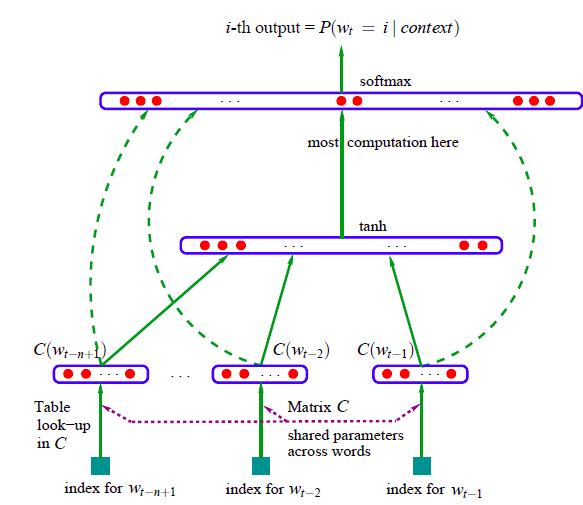
\includegraphics[width=15cm,height=12cm,keepaspectratio]{files/npmodel.png}
	\caption{Neural Probabilistic Model (\cite{bengio2003neural})}
	\label{fig:npm}
\end{figure}
The first layer is an embedding layer, which generates word embeddings by multiplying an index vector with a word embedding matrix. In the middle, there are one or more layers that produce an intermediate representation of the input. Such a layer may be a fully-connected layer that applies a non-linearity to the concatenation of word embeddings of $n$ previous words thus taking context in consideration. The final layer is a softmax layer which produces a probability distribution over words in the vocabulary, $\mathbf{V}$ and thus supplying with a prediction of the word.\\
\cite{bengio2003neural} reported that their approach has achieved significant improvement on state-of-the-art n-gram models, meanwhile taking the advantage of longer contexts.

\subsection{Distributive Word Representation}\label{w2v}
In their paper, \cite{mikolov2013efficient} introduced a technique to learn word vectors from a huge data corpus which contains billions of words. They have proposed two new model architecture for learning the distributed representation of the words. Besides the models, \cite{mikolov2013efficient} also proposed some techniques to determine similarity measures between words. The two models are known as Continuous Bag-of-Words Model and Continuous Skip-gram Model. The models are trained on dataset of size $N$ with vocabulary size $V$ to generate the vectors of dimension $D$. 
A brief description of these models are as follows:
\subsubsection{Continuous Bag-of-Words Model (CBOW)}
The model, introduced by \cite{mikolov2013efficient}, tries to predict the current word based on its context words. This model is very similar to the feedforward NNLM, but uses a continuous distributed representation of context instead of bag-of-words. They also stated that the training time complexity of the model is:
\begin{equation}
Q = N \times D + D \times \log_2(V)
\end{equation}
\subsubsection{Continuous Skip-gram Model}
Another model proposed by \cite{mikolov2013efficient}, is similar to CBOW but it tries to maximize classification of a word based on the words in the same sentence. In other words, the model predicts the context words given their center word. Here distance of words to the input word, represented by $C$, also comes in play. This distance is important since the more distant words are less related to the center word. So one can assign less weight to distant context words thus helps to attain better context words. They also stated that the training time complexity of the model is:
\begin{equation}
Q = C \times (D+D\times\log_2(V))
\end{equation}
Both the models became very popular because of their simple and shallow architecture. They are easy to train and generate high quality word vectors.
\subsection{Global Vectors(gloVe)}
In this paper, \cite{pennington2014glove}, proposed an alternative model to generate word embeddings. They proposed to use the statistics of word co-occurrences in a corpus. They tried to explore the relationship between words using these statistics. They referred to the model as GloVe, "Global vectors", as the model explores the global corpus statistics.\\
\\
It is a log-bilinear model with a weighted least-squares as an objective function. The main idea that the model follows is to find the ratios of word-word co-occurrence probabilities. These ratios have the potential to encode some form of meaning. In other words, similar meaning words have a high ratio of co-occurrence.\\
The authors reported that the model performed better than the state of art models for word analogy, word similarity and named entity recognition tasks. The model introduced a new weighted least square regression model. This is done by using a weighing function $\mathit{f(\mathbf{X}_{ij}})$ in cost function.
\begin{equation}\label{eq:J}
\mathit{J = \sum_{i,j=1}^{v} f(X_{ij})(w_i^T \tilde{w_j}+b_i+\tilde{b_j}-log X_{ij})^2}
\end{equation}
In this equation, \ref{eq:J},\\
$\mathbf{\mathit{X_{ij}}}$ denotes number of times word \textit{j} occurs in context of word \textit{i}\\
$\mathit{w \in \mathbf{R}^d}$ are word vectors.\\
$\mathit{\tilde{w} \in \mathbf{R}^d}$ are separate context word vectors.\\ 
$\mathit{b_i, \tilde{b_j}}$ are biases.\\
$\mathbf{V}$ is the vocabulary size.\\
$\mathit{f(x)}$ function that worked well in this model is:
\begin{center}
	$$
	f(x) = \left\{
	\begin{array}{ll}
	(x/x_{max})^\alpha & \quad x < x_{max} \\
	1 & \quad otherwise
	\end{array}
	\right.
	$$
\end{center}
\subsection{Word vectors using FastText}
The approach followed in this technique is the most related approach to our proposed model in this thesis. \cite{bojanowski2016enriching} proposed a model which is basically an extension of skip-gram model, \cite{mikolov2013efficient}. In this approach, the model learns the representations of sub words in addition to the words in the vocabulary. Thus the main focus of this approach is to include the morphology of words.\\
The model used in this approach is also known as Sub-word model. The main difference between this model and the skip gram model is the scoring function \textit{s}. This different scoring function, takes into account the morphological information of the words.
Each word is represented as a bag of character \textit{n}-gram. The word \textit{w} is also considered in the set. The example for the set for the word "machine" with \textit{n} = 3 include:
\begin{center}
	$\mathit{<ma, mac, ach, chi, hin, ine, ne>, <machine>}$
\end{center}
The vector for the word \textit{w} represented by $\mathbf{z_{\mathit{g}}}$ to each $\mathit{n}$-gram $\mathit{g}$ will have scoring function:
\begin{equation}
\mathit{s(w,c)} = \sum_{g\in \mathcal{G}_{\mathit{w}}} \mathbf{z}^T_{\mathit{g}}\mathbf{v}_{\mathit{c}}
\end{equation}
This is a very simple model which allows sharing the representation across words. Such approaches help in learning vector representation of rare words.\\
One drawback in this approach is that training is slower than the training of a skip gram model. On the other hand, it has also been reported that the morphological information significantly improves the syntactic tasks, as the accuracy surpassed the base line. The performance of proposed model seems to quickly saturate where as the CBOW's performance improved significantly when the data size is increased. But the most important result from the proposed approach is that very good word vectors are generated using a very small training dataset. 
